%\documentclass [12pt] {article}
\documentclass [12pt, a4paper, titlepage]{article}
\usepackage{graphicx}
\usepackage{latexsym}
\usepackage{color}
\usepackage{float}
\usepackage[pdftex,colorlinks,linkcolor=black,anchorcolor=red,citecolor=green]{hyperref}
    \author{Robert}
    \title{\textbf{How to use MonorailTest script}}
\date{2015/06/28}

\setlength{\abovecaptionskip}{0pt}
\setlength{\belowcaptionskip}{10pt}

\begin{document}
%\linespread {1.2}
\maketitle

\tableofcontents
\clearpage

\section{Purpose}
\paragraph[indent]{}The original purpose of this utility is used to test hardware simualtion environment with Onrack Monorail APIs. So this utility  doesn't guarantee all Monorail APIs were implemented.

\section{Running the utility}
\paragraph[indent]{}You should have a linux working envrionment, and have python installed. Then copy the utility to your workspace, and decompress the utility,  and then run: \\\\
    \textbf{\textcolor{blue}{\# python mtc.py}}
    \paragraph{\textcolor{red}{Note:}} This uitility doesn't work in windows environment.

\section{Logging}
\paragraph[indent]{} When run this utility, the data including node information, DHCP information will be saved in folder data/*.txt. and the runtime log were logged in the monorailtest.log
\section{Commands}
\subsection{list command}
        \begin{description}
            \item[\textcolor{blue}{list}] List all nodes. See Figure \ref{list}
        \end{description}

         \begin{figure}[H]
         \begin{center}
         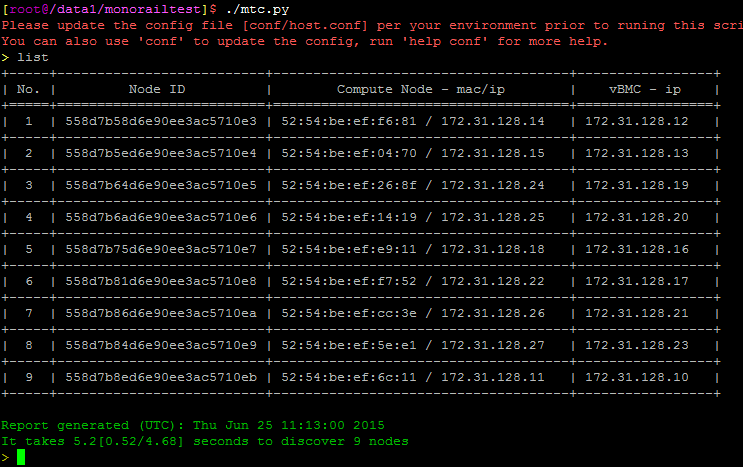
\includegraphics[width=15cm,height=10cm]{png/list.png}
         \end{center}
         \caption{List all nodes}
         \label{list}
         \end{figure}

        \begin{description}
            \item[\textcolor{blue}{list failed}] List all nodes without BMC info
        \end{description}

\subsection{delete command}
        \begin{description}
            \item[\textcolor{blue}{delete}] Delete all nodes discovered by OnRack
        \end{description}

        \begin{description}
        \item[\textcolor{blue}{delete $<node\ id>$}] Delete specific node per node id \footnote{use last 4 characters to represent whole node id string. E.g. 10eb indicates 558d7b8ed6e90ee3ac5710eb}
        \end{description}

\subsection{lookups command}
        \begin{description}
            \item[\textcolor{blue}{lookups}] Show all DHCP info for nodes including DHCP ID, mac address and IP address. See Figure \ref{lookups_fig}
        \end{description}

        \begin{figure}[H]
        \begin{center}
        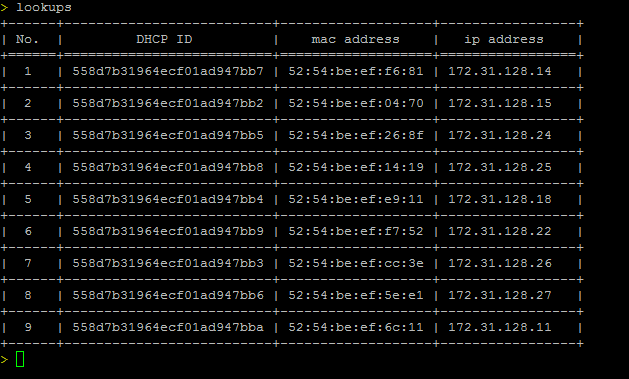
\includegraphics[width=13cm,height=10cm]{png/lookups.png}
        \end{center}
        \caption{List DHCP info for all nodes}
        \label{lookups_fig}
        \end{figure}

        \begin{description}
            \item[\textcolor{blue}{lookups id $<node\ id>$}] Lookup dhcp info per node id. See Figure \ref{lookups_fig2}
        \end{description}


        \begin{description}
            \item[\textcolor{blue}{lookups mac $<mac>$}] Lookup dhcp info per mac address. See Figure \ref{lookups_fig2}
        \end{description}

        \begin{figure}[H]
        \begin{center}
        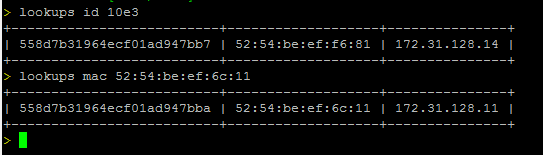
\includegraphics[width=13cm,height=4cm]{png/lookups2.png}
        \end{center}
        \caption{Lookup DHCP info  with node id and mac address}
        \label{lookups_fig2}
        \end{figure}

\subsection{catalogs command}

        \begin{description}
            \item[\textcolor{blue}{catalogs}] Show all nodes catalogs data
        \end{description}

        \begin{description}
            \item[\textcolor{blue}{catalogs $<node\ id>$}] Show specific node catalogs data per node id
        \end{description}

        \begin{description}
            \item[\textcolor{blue}{catalogs $<node\ id>$ $<source>$}] Show node catalogs data per node id and source \footnote{source could be 'dmi', 'lsall', 'lspci', 'lshw' and etc. Reference onrack document for more info.}. See \ref{catalogs}.
        \end{description}

        \begin{figure}[H]
        \begin{center}
        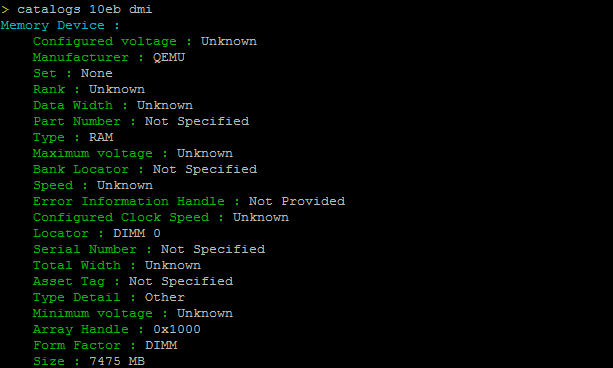
\includegraphics[width=13cm,height=9cm]{png/catalogs.png}
        \end{center}
        \caption{catalog data per node id and source 'dmi'}
        \label{catalogs}
        \end{figure}


\subsection{workflow command}

        \begin{description}
            \item[\textcolor{blue}{workflow list}] Show all available workflows. See Figure \ref{workflows1}
        \end{description}
        \begin{figure}[H]
        \begin{center}
        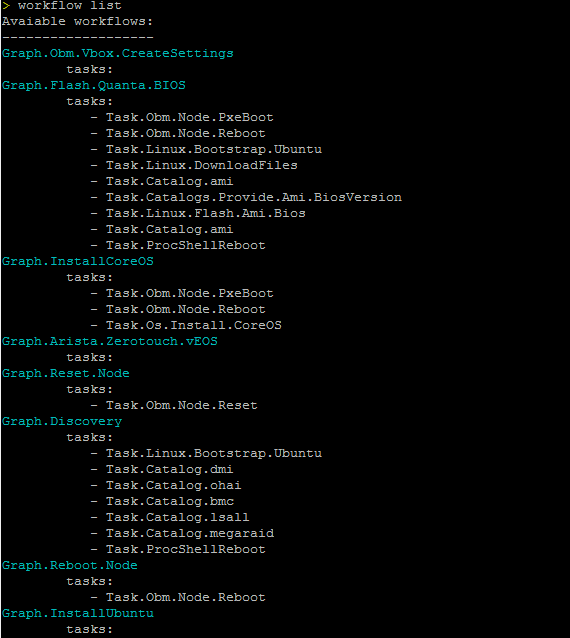
\includegraphics[width=13cm,height=15cm]{png/workflows1.png}
        \end{center}
        \caption{List all available workflows}
        \label{workflows1}
        \end{figure}

        \begin{description}
            \item[\textcolor{blue}{workflow get $<node\ id>$}] Get workflow for specific node per node id. See Figure \ref{workflows2} for example
        \end{description}
        \begin{figure}[H]
        \begin{center}
        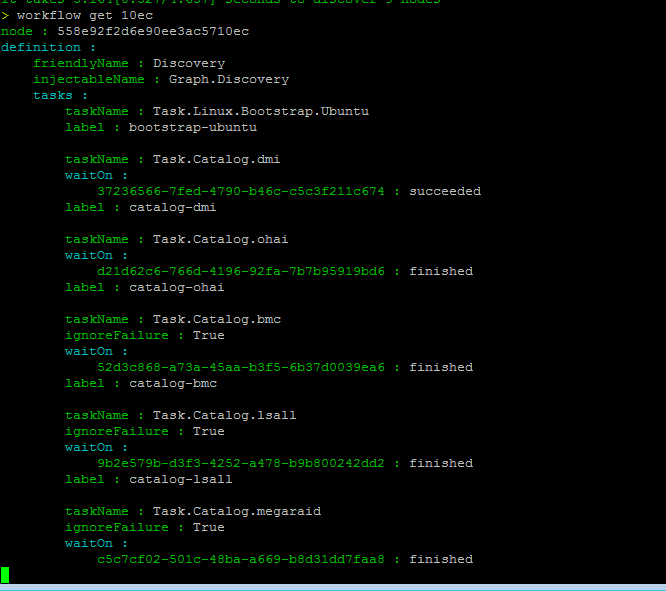
\includegraphics[width=13cm,height=14cm]{png/workflows2.png}
        \end{center}
        \caption{Get Node Workflow}
        \label{workflows2}
        \end{figure}


        \begin{description}
            \item[\textcolor{blue}{workflow set $<node\ id>$ $<action>$}] Set workflow for specific node per node id. See Figure \ref{workflows3} for example
        \end{description}
        \begin{figure}[H]
        \begin{center}
        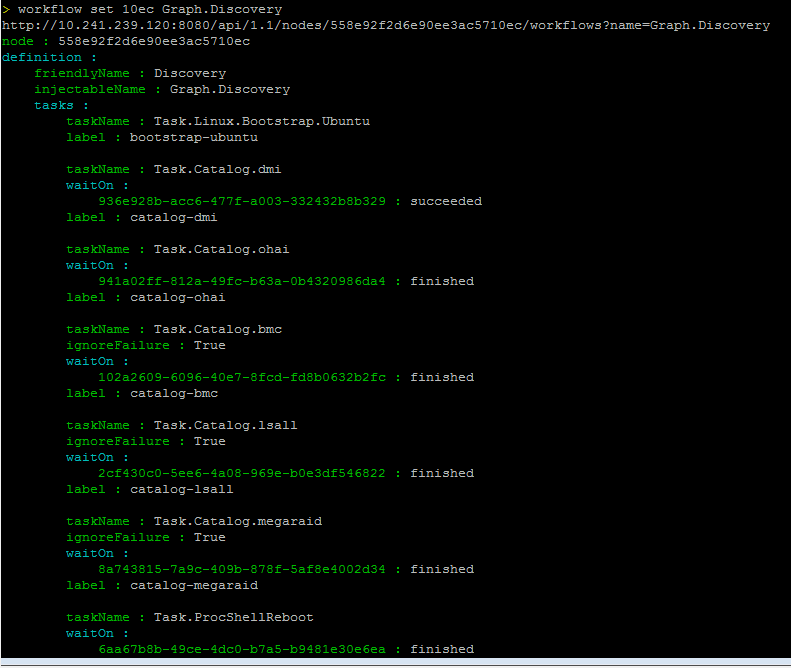
\includegraphics[width=13cm,height=14cm]{png/workflows3.png}
        \end{center}
        \caption{Run Discovery Workflow}
        \label{workflows3}
        \end{figure}


        \begin{description}
            \item[\textcolor{blue}{workflow active $<node\ id>$}] Get active workflow for specific node per node id. See Figure \ref{workflows4} for example
        \end{description}
        \begin{figure}[H]
        \begin{center}
        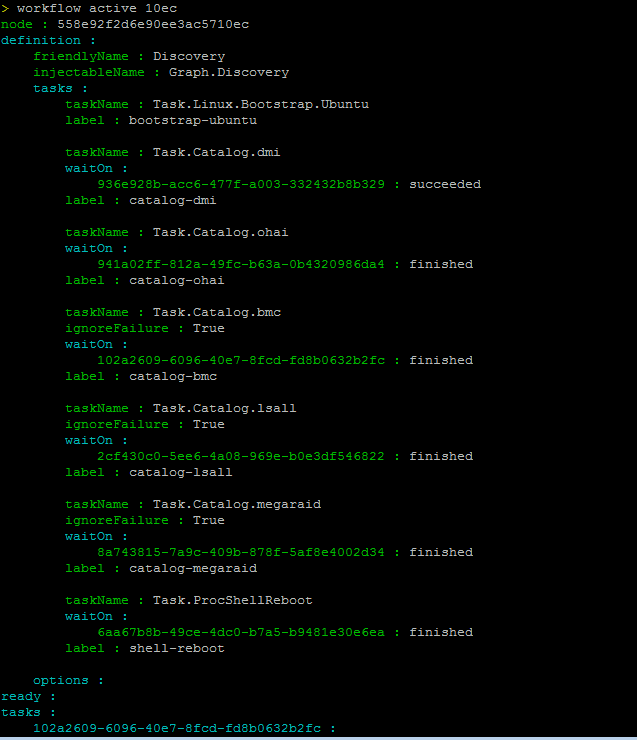
\includegraphics[width=14cm,height=17cm]{png/workflows4.png}
        \end{center}
        \caption{Get Active Workflow}
        \label{workflows4}
        \end{figure}


        \begin{description}
            \item[\textcolor{blue}{workflow delete $<node\ id>$}] Delete workflow for specific node per node id. See Figure \ref{workflows5} for example
        \end{description}
        \begin{figure}[H]
        \begin{center}
        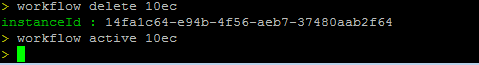
\includegraphics[width=13cm,height=2cm]{png/workflows5.png}
        \end{center}
        \caption{Run Delete Workflow}
        \label{workflows5}
        \end{figure}


\subsection{getobm command} 
        \begin{description}
            \item[\textcolor{blue}{getobm $<node\ id>$}] Get OBM settings for specific node per node id. See Figure \ref{getobm} for example
        \end{description}
        \begin{figure}[H]
        \begin{center}
        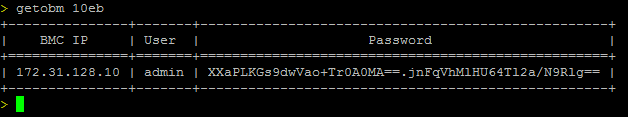
\includegraphics[width=10cm,height=3cm]{png/getobm.png}
        \end{center}
        \caption{Get OBM Settings}
        \label{getobm}
        \end{figure}

\subsection{setobm command} 
        \begin{description}
            \item[\textcolor{blue}{setobm $<node\ id>$ $<host>$ $<user>$ $<password>$}] Set OBM settings for specific node per node id. 
        \end{description}

        \paragraph[ident]{\textcolor{red}{Note:}} Basically you don't need to set the OBM manually, once a new node was discovered, the script will extract the BMC info from the catalog data, and then set the OBM automatically.

\subsection{getvm command}
        \begin{description}
            \item[\textcolor{blue}{getvm id $<node\ id>$}] Get VM name per node id. See Figure \ref{getvm} for example
        \end{description}

        \begin{figure}[H]
        \begin{center}
        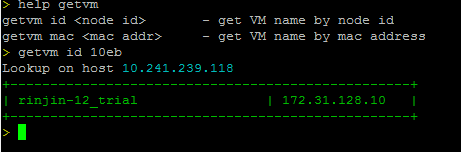
\includegraphics[width=13cm,height=5cm]{png/getvm.png}
        \end{center}
        \caption{Get VM Name}
        \label{getvm}
        \end{figure}

        \begin{description}
            \item[\textcolor{blue}{getvm mac $<mac>$}] Get VM name per mac address.
        \end{description}

\subsection{vmpower command}
        \begin{description}
            \item[\textcolor{blue}{vmpower $<action>$ $<VM\ name>$}] Control the VM. See Figure \ref{vmpower}
                \paragraph {action}:
                \begin{enumerate}
                    \item[-] reset
                    \item[-] reboot
                    \item[-] on
                    \item[-] off
                    \item[-] getstate
                \end{enumerate}
        \end{description} 

        \begin{figure}[H]
        \begin{center}
        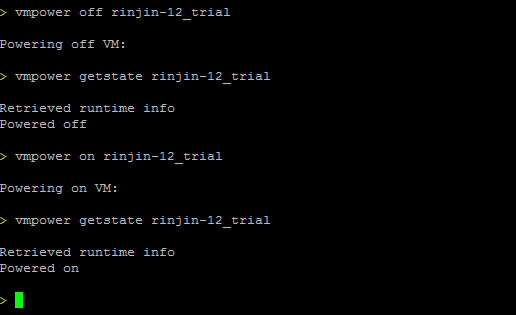
\includegraphics[width=13cm,height=8cm]{png/vmpower.png}
        \end{center}
        \caption{VM Power Control}
        \label{vmpower}
        \end{figure}

\subsection{versions command}
        \begin{description}
            \item[\textcolor{blue}{versions}] List all component versions of OnRack. Refer to Figure \ref{versions}
        \end{description}
        \begin{figure}[H]
        \begin{center}
        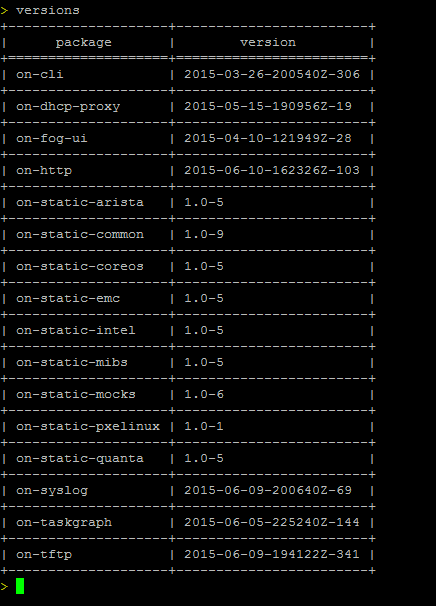
\includegraphics[width=10cm,height=18cm]{png/versions.png}
        \end{center}
        \caption{List all versions}
        \label{versions}
        \end{figure}


\subsection{conf command}
        \begin{description}
            \item[\textcolor{blue}{conf list}] List current configuration. See Figure \ref{conflist}
        \end{description}

        \begin{figure}[H]
        \begin{center}
        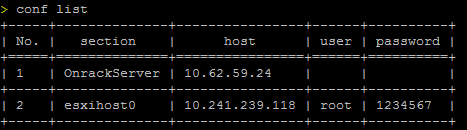
\includegraphics[width=13cm,height=4cm]{png/conflist}
        \end{center}
        \caption{Conf List}
        \label{conflist}
        \end{figure}

        \begin{description}
            \item[\textcolor{blue}{conf update $<section>$ $<option>$ $<value>$}] Update specific option for section. See Figure \ref{confupdate}
        \end{description}

        \begin{figure}[H]
        \begin{center}
        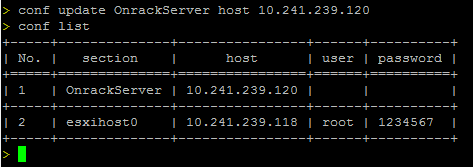
\includegraphics[width=13cm,height=5cm]{png/confupdate}
        \end{center}
        \caption{Conf Update}
        \label{confupdate}
        \end{figure}


        \begin{description}
            \item[\textcolor{blue}{conf add $<section>$ $<host>$ $<user>$ $<password>$}] Add a section. See Figure \ref{confadd}
        \end{description}

        \begin{figure}[H]
        \begin{center}
        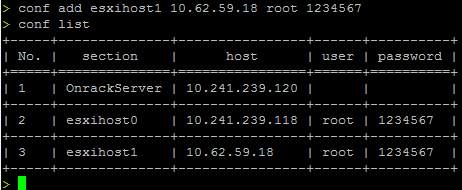
\includegraphics[width=13cm,height=5cm]{png/confadd}
        \end{center}
        \caption{Conf Add}
        \label{confadd}
        \end{figure}

        \begin{description}
            \item[\textcolor{blue}{conf del $<section>$}] Delete a section. See Figure \ref{confdel}
        \end{description}

        \begin{figure}[H]
        \begin{center}
        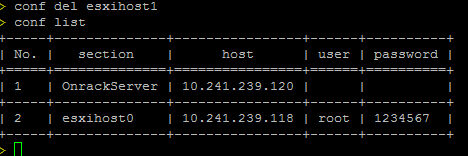
\includegraphics[width=13cm,height=5cm]{png/confdel}
        \end{center}
        \caption{Conf Del}
        \label{confdel}
        \end{figure}

        \begin{description}
            \item[\textcolor{blue}{conf load}] Load configuration
        \end{description}

        \paragraph{\textcolor{red}{Note:}} Once you change the configuration, you should run 'conf load' to take the configuration effect.

\subsection {lsdhcp command}
        \begin{description}
            \item[\textcolor{blue}{lsdhcp all}] List all IPs allocated by the DHCP server on OnrackServer
        \end{description}

        \begin{description}
            \item[\textcolor{blue}{lsdhcp active}] List current active IPs allocated by the DHCP server on OnrackServer
        \end{description}
        
\subsection {shell command}
         \paragraph[indent]{} You could run shell command with this application. E.g.\\
         Running '\textbf{\textit{ls -l}}' shell command like this: \\\\
         \textcolor{blue}{$>$ !ls -l} \\\\
         Refer to figure \ref{shell}

         \begin{figure}[H]
         \begin{center}
         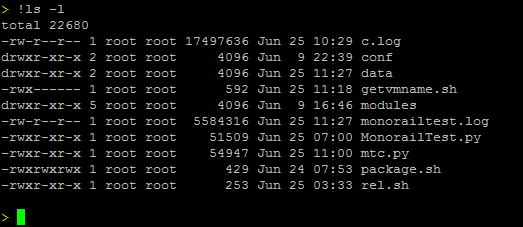
\includegraphics[width=13cm,height=6cm]{png/shell}
         \end{center}
         \caption{Run 'ls -l' command}
         \label{shell}
         \end{figure}


\subsection {onconfig command}
        \begin{description}
            \item[\textcolor{blue}{onconfig get}] Get onrack server configurations. Refer to Figure \ref{onconfig}
        \end{description}

         \begin{figure}[H]
         \begin{center}
         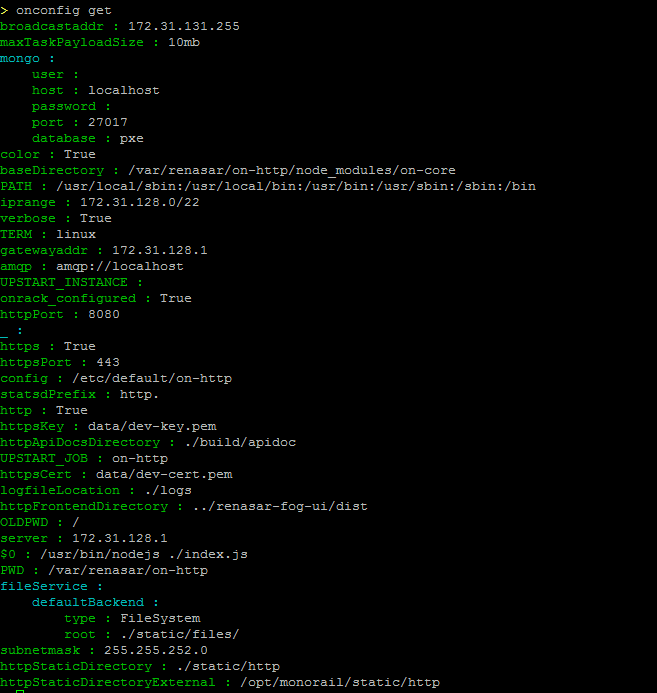
\includegraphics[width=13cm,height=15cm]{png/onconfig}
         \end{center}
         \caption{onconfig command}
         \label{onconfig}
         \end{figure}



\subsection {quit command}
        \begin{description}
            \item[\textcolor{blue}{quit}] Quit the application.
        \end{description}

\subsection {help command}
        \begin{description}
            \item[\textcolor{blue}{help}] List all available commands. Refer to Figure \ref{help}
            \item[\textcolor{blue}{help $<command>$}] Help command. e.g help getvm. See Figure \ref{help}
        \end{description}

        \begin{figure}[H]
        \begin{center}
        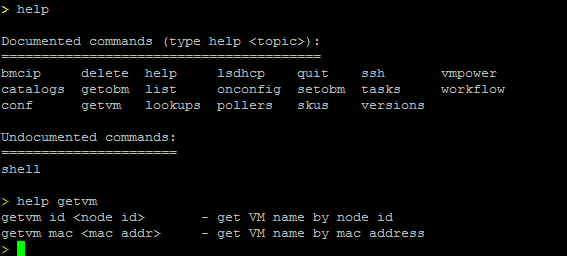
\includegraphics[width=13cm,height=8cm]{png/help}
        \end{center}
        \caption{Help}
        \label{help}
        \end{figure}

\end{document}
